
\documentclass[12pt,a4paper]{article}

\usepackage{pdflscape}
\setlength{\textwidth}{165mm}
\setlength{\textheight}{235mm}
\setlength{\oddsidemargin}{-0mm}
\setlength{\topmargin}{-10mm}

\usepackage{mathtools}
\DeclarePairedDelimiter\abs{\lvert}{\rvert}%
\DeclarePairedDelimiter\norm{\lVert}{\rVert}%
% Swap the definition of \abs* and \norm*, so that \abs
% and \norm resizes the size of the brackets, and the
% starred version does not.
\makeatletter
\let\oldabs\abs
\def\abs{\@ifstar{\oldabs}{\oldabs*}}
%
\let\oldnorm\norm
\def\norm{\@ifstar{\oldnorm}{\oldnorm*}}
\makeatother

\newcommand*{\Value}{\frac{1}{2}x^2}%
%\usepackage{graphicx}
\usepackage{graphicx}
\usepackage{subfigure}%exclusive to subcaption
%\usepackage{subcaption, float} 
\usepackage{xcolor}
\definecolor{ggray}{RGB}{47,79,79}
\definecolor{firebrick}{RGB}{178,34,34}
\definecolor{green1}{RGB}{50,205,50}
\definecolor{umbrella}{RGB}{0,191,255}

\usepackage{pgfplots}
\usepackage{tikz}
\usetikzlibrary{patterns,arrows,shapes,positioning,shadows,trees}
\tikzstyle{every node}=[draw=black,thick,anchor=west]
\tikzstyle{selected}=[draw=red,fill=red!30]
\tikzstyle{optional}=[dashed,fill=gray!50]
\tikzstyle{neglected}=[dashed]

\usepackage{amsfonts}
\usepackage{amssymb,amsmath} %  $\displaystyle \sum$ will print a bigger one Σ , like in equations  in amsmath package

\DeclareMathOperator{\sgn}{sgn}

\usepackage{soul}

\usepackage{titlesec}
\titleformat*{\section}{\Large\sffamily}
\titleformat*{\subsection}{\large\sffamily}
\titleformat*{\subsubsection}{\itshape \sffamily}


%\renewcommand{\refname}{參考文獻}
\usepackage[nottoc]{tocbibind}
%\settocbibname{參考文獻}

\usepackage{multirow}
\usepackage{booktabs}
%\usepackage[square]{natbib}

\title{Numerical Analysis HW06: Conjugate Gradient Method}
\author{Ming-Chang Chiu}
\date{\today}
\begin{document}
\maketitle
\fontsize{12}{20pt}\selectfont %本行指令第一個12是字體大小、第二個20是行距,selectfont一定要加才會發生效果。但此指令只對正文有效,註解無效

\section{Objective}
The objective of Conjugate Gradient Method(a.k.a. CGM) is to find the minimum solution of a linear system iteratively as efficient as possible. In this homework, we are supposed 
to solve multiple resistor networks like the following figure using CGM but with different resistors per side, get corner voltages and equivalent resistance, and then compare the results with the those of hw04.cpp, which is implemented with LU decomposition.
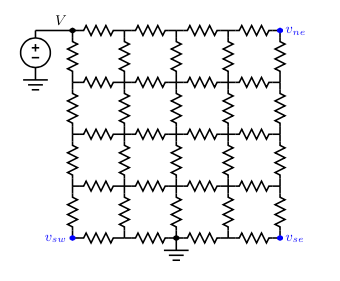
\includegraphics[scale =0.6 ]{./sample1.png}
\section{Workflow}

\begin{description}  

\item [Usage:] For example, ./hw06.out $num$. $num$ is the number of resisters per side and it could be any number, but even number is preferred. %For $num = 2, 4, 10, 20$, the resistance would be the same as the 
%one in HW04 and the default resistance is $100Ohms$.
\item [Form matrix:] For linear system $Ax=b$, first build system matrix $A$ with Kirchoff node method.
\item [Modify matrix:] In order to satisfy the limitation of CGM, $A$ has to be positive definite matrix, so it is important to modify the system matrix to reach the this confinement. 
\item [Initialize RHS:]Since LHS is modified, RHS shall simultaneously be assigned accordingly so that the linear system stay equivalent to the original one.
\item [Solve:] Eventually, use CGM to solve the linear system.

\end{description}

\section{Results}

\begin{tabular}{|c|c|c|c|c|c|c|}
\hline  Resistors Per Side & Iteration number  & $Vne(V)$  & $Vsw(V)$ & $Vse(V)$  & Time(s) & $Req(Ohm)$ \\
\hline    2    		& 9     	& 0.482759 & 0.275862 & 0.172414  & 0  	& 1208.333333  \\
\hline    2(hw4)    & N/A     & 0.482759 & 0.275862 & 0.172414  & 0	 & 1208.333333  \\
\hline    4    		& 20   	& 0.441080 & 0.280747 & 0.211722  & 0       & 850.525689    \\
\hline    4(hw4)    & N/A     & 0.441080 & 0.280752 & 0.211722  & 0.002   & 850.530303  \\
\hline    10  		& 49   	& 0.407872 & 0.293964 & 0.248430  & 0.017       & 491.202658    \\
\hline    10(hw4)    & N/A     & 0.407838 & 0.294016 & 0.248441  & 0.012 & 491.202388  \\
\hline    20  		& 96   	& 0.392841 & 0.301598 & 0.265615  & 0.401       & 307.389238    \\
\hline    20(hw4)    & N/A     & 0.392824 & 0.301635 & 0.265600 & 0.510  & 307.389274  \\
\hline    40  		& 184 	& 0.382571 & 0.307028 & 0.277334  & 19.540     & 185.644983    \\
\hline    40(hw4)    & N/A     & 0.382576 & 0.307032 & 0.277288  & 28.149  & 185.645028  \\
\hline    50  		& 226 	& 0.379942 & 0.308437 & 0.280325  & 64.904     & 156.853212    \\
\hline    50(hw4)    & N/A     & 0.379957 & 0.308423 & 0.280271 & 104.032  & 156.853262  \\
\hline    100		& 426 	& 0.373215 & 0.312095 & 0.287907  & 2005.044 & 91.476893    \\
\hline    100(hw4)& N/A 	& 0.373304 & 0.311969 & 0.287845  & 6229.428 & 91.476989    \\\hline 
\end{tabular}\\

% this subplot is located at the bottom of the file, which is weird
\begin{figure}[H]
\begin{center} 
	\subfigure[b]{ \label{bird-a}
		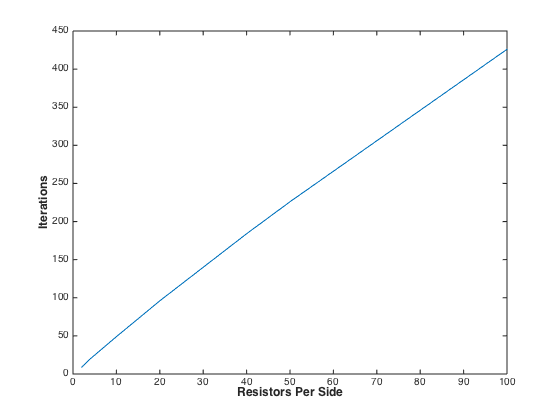
\includegraphics[scale =0.75 ]{./iter_resis.png}
		} 
	\subfigure[a]{\label{bird-b}
		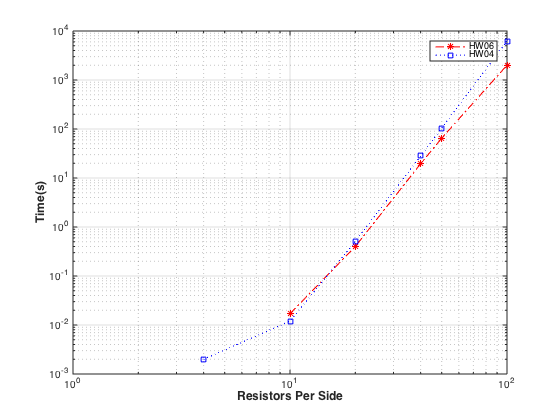
\includegraphics[scale =0.75 ]{./time_resis.png}
		} 
	\end{center}
\caption{abc}
\label{bird}
\end{figure}

	

	
% These two graphs are located correctly, right after the tabular above.
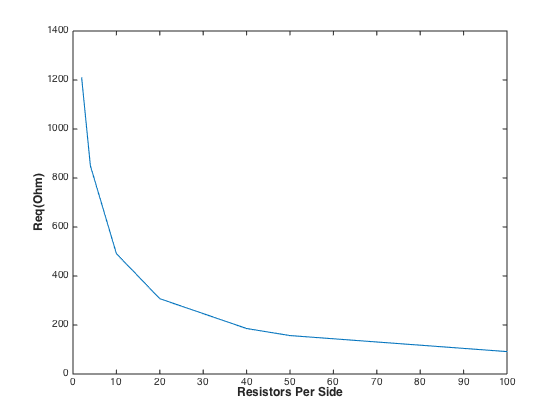
\includegraphics[scale =0.75 ]{./req_resis.png}

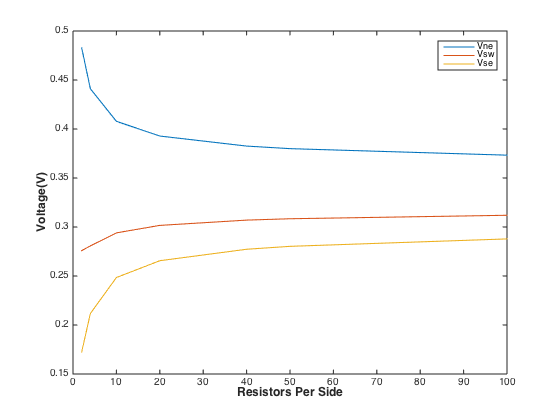
\includegraphics[scale =0.75 ]{./volt_resis.png}
	





\section{Observations}

\begin{description}

\item [Iteration:] The number of iterations of CGM for each problem is roughly linear to the resistors per side, that is, CGM is highly efficient for the iterations is linear to square root of the size of matrix $A$.
\item [Node Voltage:] The voltage is at least accurate to the second digit after the decimal point; for most cases, it is precise to the third digit after the decimal point. This explains the reason why people are using CGM since the precision is acceptable. For all $Vne, Vsw, Vse$, they tend to converge while the network size expands.
\item [Time analysis:] As I have discussed, CGM is a very fast method to converge. Using CGM is normally faster than using LU method when 
tackling large amounts of variables($>100$) in the linear system. The complexity for HW4 is $O(n^{2.9974})$, calculated by $\frac{log(28.149) - log(0.510)}{log((40+1)^2) - log((20+1)^2)}$, and the 
counterpart for HW6 is not that stable but roughly $O(n^{2.9043})$, derived from $\frac{log(19.410) - log(0.396)}{log((40+1)^2) - log((20+1)^2)}$, which means CGM has similar complexity to LU decomposition but the coefficient of the time complexity is smaller.
\item [Equivalent resistance:] The equivalent resistance tend to exponentially decrease and the inclination to convergence is high.
\item [Overall:] The precision of CGM to me is accurate enough since no matter for equivalent resistance or node voltages, the differences between HW4 and HW6 are not unacceptable. In addition, the CGM is much faster when the variables to be solved are massive. Therefore, CGM is a better choice when solving this kind of problems.
\end{description}






\end{document} 